\documentclass[10pt]{scrreprt}
\usepackage[usenames]{color}
\usepackage{amssymb} 
\usepackage{amsmath} 
\usepackage[utf8]{inputenc}
\usepackage{listings}
\usepackage{multirow}
\usepackage{biblatex}
\usepackage[T1]{fontenc}
\usepackage{scrhack}
\usepackage[table]{xcolor}
\usepackage{etoolbox}
\usepackage{pdfpages}
\usepackage[toc,page]{appendix}
\usepackage{hyperref}
\makeatletter
\patchcmd{\scr@startchapter}{\if@openright\cleardoublepage\else\clearpage\fi}{}{}{}
\makeatother

\addbibresource{bibliography.bib}

% Schmale Seitenränder festlegen
\KOMAoption{DIV}{15}

% Moderne Schriftart verwenden
\usepackage{lmodern}

% Schriftart Helvetica verwenden (Arial-ähnlich)
\usepackage{helvet}

% serifenfreie Schriftvariante verwenden
\renewcommand{\familydefault}{\sfdefault}

% Einbinden von Pixelgrafiken (JPG, PNG)
\usepackage{graphicx}

% Einbinden von Vektorgrafiken (SVG)
\usepackage{svg}

% Kopf- und Fusszeilen selbst definieren
\usepackage{scrlayer-scrpage}

% Voraussetzung für biblatex
\usepackage{csquotes}

\title{Optimizing a Train Network --- A Comparison of Two Methods\\
\begin{figure}
    \begin{center}
        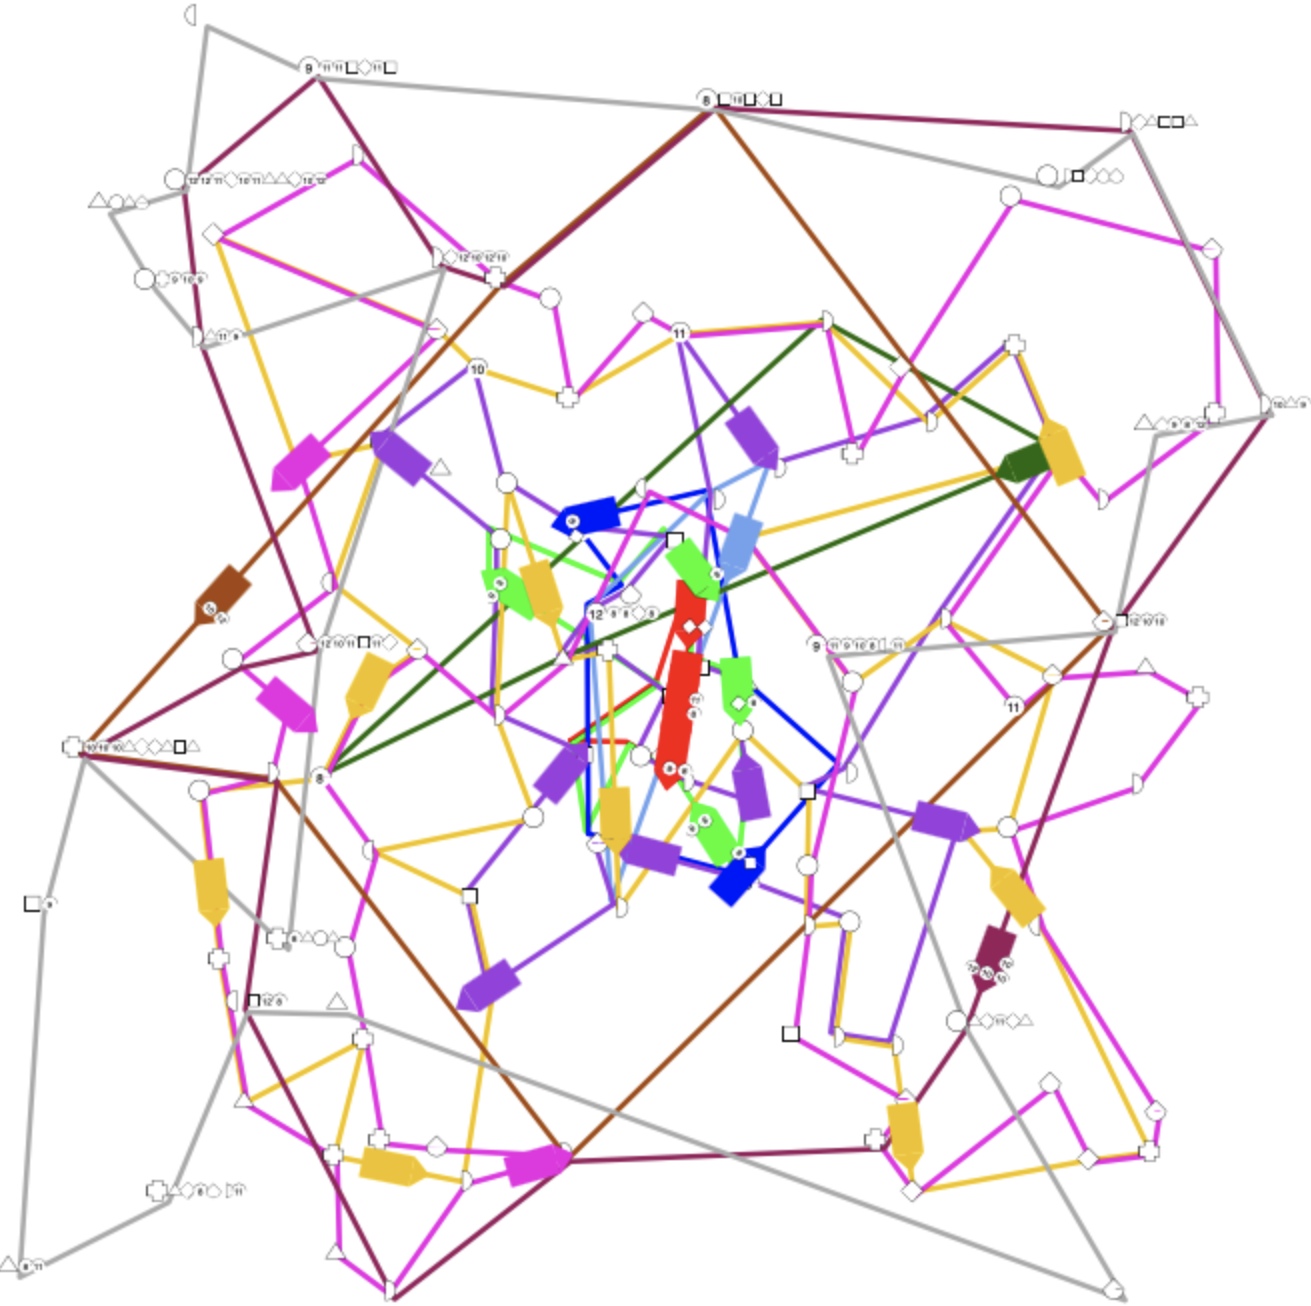
\includegraphics[scale=0.48]{pictures/simulation_picture.png}
    \end{center}
    \label{Visualization (title image)}
\end{figure}
}
\author{Written by Ema Skottova\\
Supervised by Stefan Rothe}

\date{Berne, November 2020}


\publishers{\vspace{1cm}
\includegraphics[scale = 0.15]{pictures/logo.png}\vspace{0.4cm}\\
Gymnasium Kirchenfeld\\
Department of Mathematics and Natural Sciences\\
M21a}

% selbstdefinierte Kopf- und Fusszeile verwenden
\pagestyle{scrheadings}

\lohead{
\includegraphics[scale=0.06]{pictures/logo.png} Matura Project}
\cohead{Optimizing a Train Network}
\rohead{Ema Skottova}
\cofoot{\thepage}
%

\begin{document}
\maketitle


\chapter{Abstract}
The idea of this paper was to compare the ability of two optimization methods to optimize a train network. The considered methods are simulated annealing and genetic algorithms. In order to do this, the train network problem was generalized and a general solution, which depends on the values of some parameters, was written. The optimization methods were implemented and given the option to decide on values for the parameters. 80 random input files were created and the solutions the optimization methods produced to each were compared. Overall, the differences were not very large. Simulated annealing has performed slightly better than the genetic algorithm.

\newpage

\tableofcontents

\newpage

\chapter{Introduction}

Optimization problems are a part of everyday life. Whether the goal is to get from A to B as quickly as possible or to make the highest possible profit from a product, many things need to be optimized. Sometimes the number of possibilities is relatively small, sometimes it is infinite. In some cases, it might not matter which solution is chosen, in some there might be enough time available to thoughtfully evaluate all options. More and more problems require a fast way to find a good solution. Many different methods have been developed over the years to tackle these problems. The goal of this project is to compare two of these methods.

The inspiration for this project comes from my interest in the theory behind these problems as well as their potential solutions. The problem chosen for this project comes from the first round of the Swiss Olympiad in Informatics. In the first round there is always a creativity task, where it is impossible to test all solutions, but there are many approaches to reach an acceptable solution. In the fall of 2019, the task was to optimize a train network. During the first round, I only submitted a simple solution which solved a special case of the problem.

\begin{figure}[h]
    \centering
    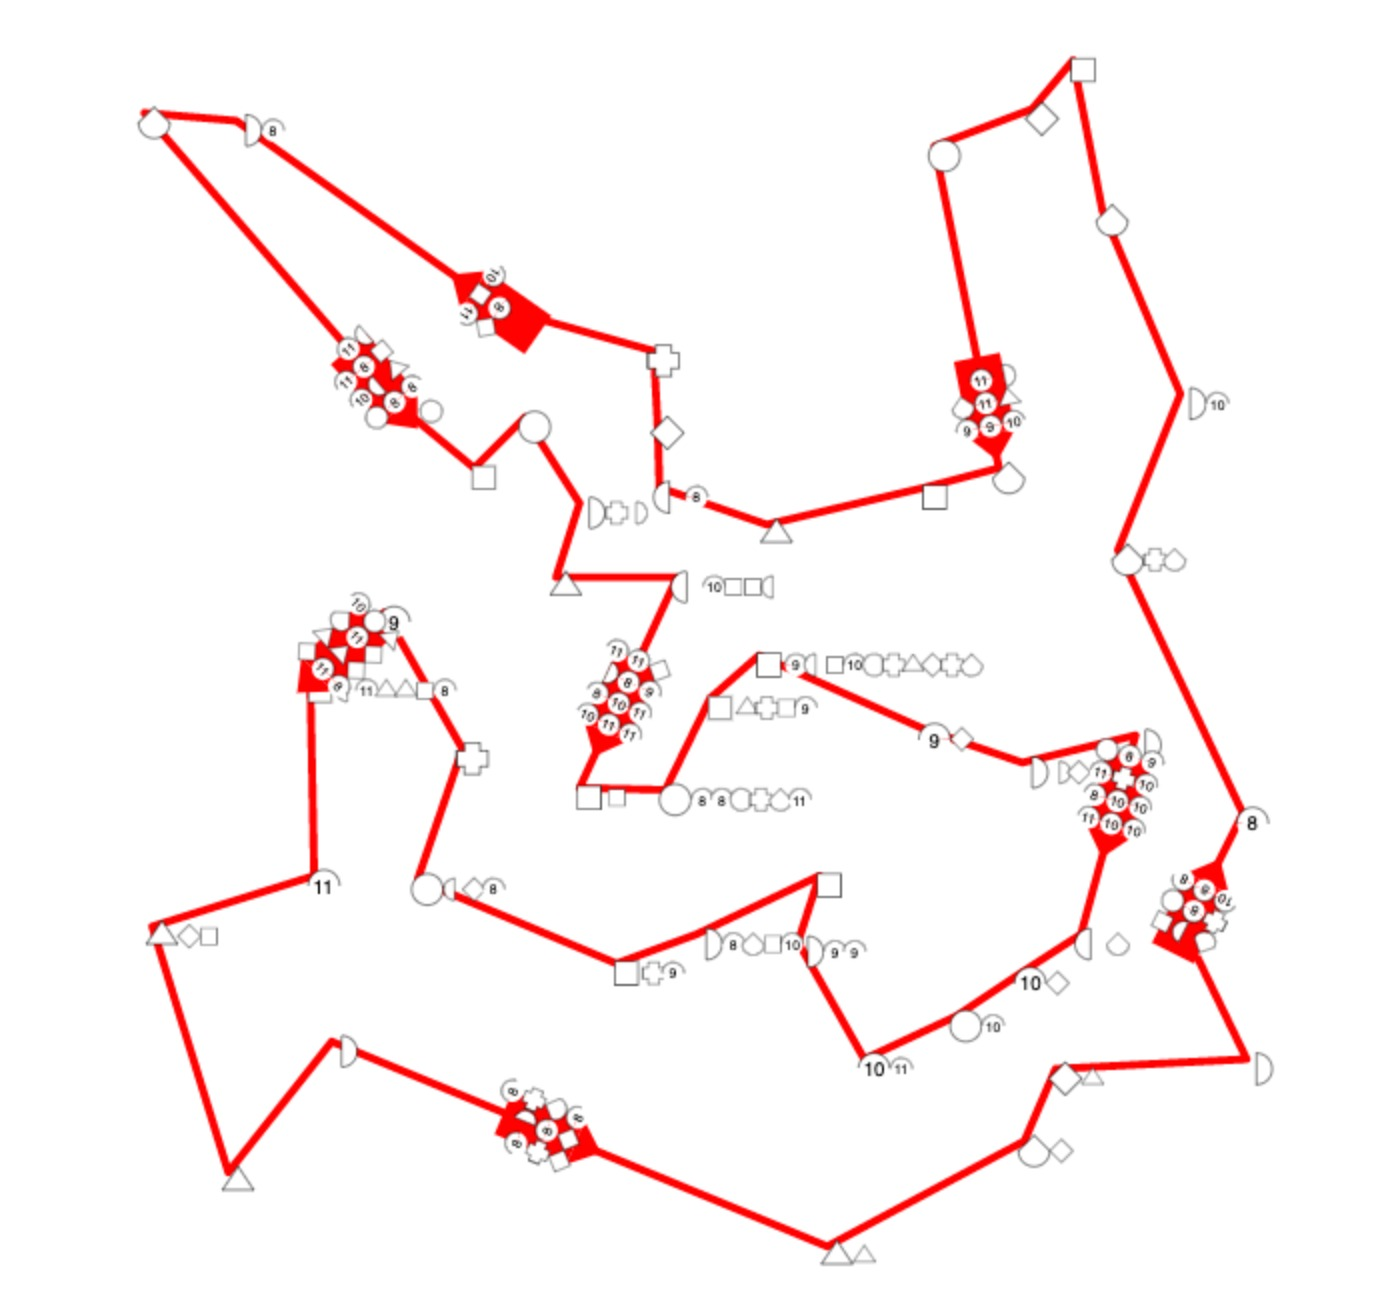
\includegraphics[scale=0.2]{pictures/sub2.jpeg}
    \caption{Solution for a special case}
    \label{}
\end{figure}

The optimization methods chosen for this project are simulated annealing and genetic algorithms. Simulated annealing is based on the idea of a cooling metal while genetic algorithms try to mimick evolution. I have first encountered the former at a programming camp and the latter was suggested by my supervisor.

\chapter{Objectives}

The project is split into two parts. The first part consists of programming a general solution to the train network problem and the second deals with the comparison of the two optimization methods. The objective of the first part is to have a working program in which the two optimization methods optimize solutions. The goal of the second part is to compare the two optimization methods.


\chapter{Theoretical Background}

\section{Optimization Problems}
In an optimization problem the objective is to find the best (optimal) solution. Example problems include finding the minimum/maximum of a mathematical function, the shortest train connection between two cities, a way to maximize the profit of a company, or the optimal shape for a vehicle. In applied mathematics or outside of mathematics, the term often refers to problems where it is difficult to find the optimal solution. Therefore, instead of looking for the optimal solution, the objective becomes finding a sufficiently good one. In this project, that type of problem is considered.

Mathematically, a solution can be modelled using a set of parameters, which unambiguously define the solution. A value function is needed to compare different solutions. 

To better understand what this means the terms will be explained using the example of a company that is trying to optimize the profit they can make from a certain product. The parameters for the product would be its size, color, and types of components. Once those are defined, it is clear what the product will look like. To compare the value of different types of products, the company will have to decide on a way to evaluate them. The value of a product will depend on the price of its production, the price at which it is sold and the number of times it can be sold. The profit the company can make off the product will be the difference of the selling price of the product and the price to produce it multiplied by the number of times the product can be sold.

\section{Optimization Methods}
An optimization method is a procedure to find the optimal (or a sufficiently good) solution.

\subsection{Brute-Force}
One method which is sometimes used for optimization problems is called brute-force. When brute-force is used, all possible solutions are computed and the best one is chosen in the end. This method always finds the best solution because it considers every possible solution. Calculating all possible solutoins also has its downsides. The main issue with this method is that it is often too slow. This happens because it has to compute too many similar things many times and it does not terminate even if it is clear that a solution will be bad.

\subsection{Greedy}
A greedy algorithm always takes the best local option. This method is good at finding a local optimum (no similar solution is better). A greedy algorithm does not consider solutions that are worse than the best solution it already has. This is a problem because it is sometimes necessary to explore some solutions that look bad to find the optimal one. The main downside of this method is that it gets stuck in local optima and only considers a small number of different solutions.

\subsection{Properties of Better Methods}
Neither brute-force nor greedy algorithms seem to be very useful for solving problems with too many possible solutions. Brute-force would take too long and a greedy algorithm would just find some solution, without considering most options. Nevertheless, both approaches have some strengths. The goal of a good optimization method is to combine the strengths of both methods while avoiding their weaknesses as much as possible. In practice, this means using the fact that some solutions are better than similar ones just like a greedy algorithm, without computing all the bad ones like it is done with brute-force. Similarly, a diverse range of different solutions should be considered, just like it is done with brute force.

\section{Simulated Annealing}
Simulated annealing is the first of the two methods chosen for this project. The main idea comes from metallurgy, where metals need to be cooled slowly to ensure that the atoms are arranged in the most stable way they can be. At first, the single atoms are moving around very quickly trying out different arrangements to come to a state of lower energy. The cooler the metal gets, the slower the atoms move. Towards the end, only small changes are made to the arrangement and the atoms only move if it immediately leads to a state with lower energy.

The optimization method based on this idea goes as follows: First, a random solution is chosen and the temperature is set to an initial value. Then, until the temperature has cooled off to a predefined value, a neighboring solution (a solution that is very similar to the current one) is chosen. If the new solution is better than the current one, it is set as the current solution. If it is not, the new solution will be accepted with a certain probability, which is based on the current temperature and how much worse the new solution is. This method was developed independently multiple times. The name was proposed by Kirkpatrick, Gelatt Jr. and Vecchi with their 1983 paper \cite{SA_1983} about the method. 

The pseudocode of this method is as follows:
\lstset {language=C++}
\begin{lstlisting}
    t = initial_temperature
    s = random_solution()
    while t >= final_temperature 
    {   
        new_s = find_neighbor(s)
        if p(new_s, s, t) > rand(0, 1)
        {
            s = new_s
        }
        temperature += step
    }
    return s
\end{lstlisting}


$initial\_temperature$, $final\_temperature$ and $step$ are defined beforehand. $find\_neighbor(s)$ should return a random solution similar to $s$. In this project, a neighbor will be a solution where only one parameter has been changed. $val(s)$ computes the value of s. Better solutions have a higher value. $p(new\_s, s, t)$ returns the probability that the new solution will be accepted. This probability is 1 if the new solution is better than $s$, otherwise the Boltzmann distribution is used. \cite{SA1} This distribution calculates how likely a state with a certain energy is at a certian temperature. It can be used to find a formula for the ratio of the probabilities of $s$ and $new\_s$.

{\Large
\begin{equation}
    e^{
    \frac{
        \epsilon_{b} - \epsilon_{n}
    }{
        kT
    }
    }
\end{equation}
}

$\epsilon_n$ is the energy of $new\_s$, $\epsilon_b$ the energy of $s$, $k$ is Boltzmann's constant and $T$ the current temperature. The energies of the solutions correspond to $-1$ times their values. This is because in the application case for which the formula was designed, a smaller energy is more likely. However, in an optimization problem the value of a solution should be maximized. The constant can be ignored in this case, as the values of the solutions have an arbitrary scale.

The formula fulfills the following necessary conditions: The probability is between 0 and 1, the probability that a solution is accepted is higher at higher temperatures or if the solution is not much worse than the best solution so far. The first one is because the exponent is always negative. The second and third conditions are satisfied because the higher the temperature or the smaller the difference between the two energies, the closer the exponent is to 0.

\section{Genetic Algorithms}
The second method used for this project is based on the biological concept of evolution. In biology the fittest individuals survive and get to reproduce. Following generations have will have traits similar to the strongest individuals of the current population. A genetic algorithm uses this idea, hoping to achieve better solutions in later generations.

Similarly to biology, there is a population containing individuals. Each individual has genes and a fitness. The population is a set of solutions. Each individual corresponds to one solution. The genes of a solution are the values of its parameters. The fitness of an individual is the value of its corresponding solution. The value of the solution is computed with a value function for optimization problem.

A genetic algorithm starts with a set of random solutions. The following steps are repeated until the differences in the gene pool become too small: $selection$, $crossing$, $mutation$, and $computation$. \cite{genalg1}

\subsection{Selection}
During selection, the parents for each individual of the next generation are chosen. They are mostly chosen at random, but fitter individuals (=better solutions) are more likely to be chosen. The probability that an individual is chosen is proportional to its fitness within its population. \cite{genalg2} If the fitness of an individual $A$ is twice the fitness of an individual $B$ within the same population, $A$ will be twice as likely to be chosen as a parent than $B$. Parents are selected by choosing a random number between 1 and the sum of the values of all solutions. Next, the values of the solutions are added up until the chosen random number or a larger one is reached. The last individual that contributed to that value is chosen as a parent. It is also ensured that the second parent is not the same as the first one by disregarding the first parent for the choice of the second one. As a consequence, the sum of all values will decrease by the value of the first parent when the second one is chosen.

Consider for example a population in which the solutions have values 5, 14, 7, and 20. Their sum is 46. To choose the first parent a random number between 1 and 46 will be chosen. For example, the random number might be 17. The first individual has a value smaller than the random number. Therefore, it is not chosen. The sum of the first two individuals is 19 which is greater than 17, therefore, the second individual is chosen. For the choice of the second parent the first parent is removed from the population. Now sum of the values is 32 and the values of the individuals are 5, 7, and 20. The second parent is now chosen the same way the first parent was chosen from the initial population.

\subsection{Crossing}
After selection, the parents of each individual in the offspring are decided on. In the next step, it is decided which traits (parameters) to take from which parent. This is done by choosing a random cutoff point. Before it, all traits are taken from the first parent, after it they are taken from the second one. The following table shows the parameter values of the offspring compared to the parents assuming the cutoff point was $c$.
\begin{table}[h]
    
\begin{center}
    \begin{tabular}{ |c|c|c|c|c|c|c|c| }
        \hline
        \rowcolor{lightgray}
        Individual & \multicolumn{7}{|c|}{Parameters} \\
        \noalign{\hrule height 1.5pt}
        \rowcolor[HTML]{A3C1E6}
        Parent 1                          & $a_1$ & $a_2$ & ... & $a_{c - 1}$ & $a_c$                          & $a_{c + 1}$                          & ...                         \\
        \hline
        \rowcolor[HTML]{E6CFA3}
        Parent 2                          & $b_1$ & $b_2$ & ... & $b_{c - 1}$ & $b_c$                          & $b_{c + 1}$                          & ...                         \\
        \hline
        \rowcolor[HTML]{A3C1E6}
        \cellcolor[HTML]{FFFFFF}Offspring & $a_1$ & $a_2$ & ... & $a_{c - 1}$ & \cellcolor[HTML]{E6CFA3} $b_c$ & \cellcolor[HTML]{E6CFA3} $b_{c + 1}$ & \cellcolor[HTML]{E6CFA3}... \\
        \hline
    \end{tabular}
\end{center}
\caption{Offspring parameters after crossing}
\end{table}

Note that genes which are closer to each other in the list of parameters are more likely to be taken from the same parent. This makes sense, as parameters influencing the same decision are closer together. If one solution performs very well due to one type of decision, it is more likely that the decision will be passed on completely to the offspring.

\subsection{Mutation}
In order to make sure the individuals do not become too similar after just a few generations, mutations are made to the offspring. For this, a set number of genes (parameter values) is changed in each generation. Multiple changes might occur on the same individual.

\subsection{Computation}
In this final step the fitness (how good a solution is) of the offspring is calculated. The best few individuals of the new generation can join the population, replacing the worst few individuals of the population. The number of new individuals that are added is equal to the number of old individuals that are removed. This ensures a constant population size.



\chapter{Methods}

For this paper, the two optimization methods were compared in their ability to optimize train networks. This chapter will contain a clearer description of the actual train network problem, the technology that has been used, and the ways the testing was conducted.


\section{Technology}
All programs were written using the programming language C++. The programming language is known to be fast, which is why it is very popular for programming competitions. It seemed like the perfect choice as the author was already familiar with many functionalities of the language.
 The written part of this project was done using LaTeX. Visual Studio Code was used both for the practical (programming) part and the writing of this paper. The choice for this tool was also based on the author's familiarity with is from different programming competitions. 
 The visualization used to visualize the solutions was provided by the Swiss Olympiad in Informatics. It was written using HTML, JavaScript, and CSS.

\section{Complete Problem Statement}

The task SOIway \cite{SOIway} from the first round of the Swiss Olympiad in Informatics 2019/2020 was chosen for this project. This chapter will explain the exact problem statement and the way the input and output has to be handled.

The program is given constants and a list of events, then it has to print actions.

\subsection{Format for Input and Output}

\subsubsection{Constants}
\begin{itemize}
    \item minimal amount of time to change a line
    \item maximal number of passengers allowed on a train
    \item maximal number of passengers allowed at a station
\end{itemize}


\subsubsection{Events}

Stations, passengers, lines, and trains appear at different times. In the input each of these events is given with the time, the object that appears, the id of that object and additional attributes that object has. Here is a table showing how objects are defined in the input:

\begin{table}[h]
    \begin{center}
    \begin{tabular}{ |c|c|c| }
        \hline
        \rowcolor{lightgray}
        Object    & Identifier & Additional Attributes                          \\
        \noalign{\hrule height 1.5pt}
        Station   & s          & x-coordinate, y-coordinate, type               \\
        \hline
        Passenger & p          & id of starting station, type of target station \\
        \hline
        Line      & l          & -                                              \\
        \hline
        Train     & z          & -                                              \\
        \hline
    \end{tabular}
\end{center}
\caption{Input format table}
\end{table}

For example "50 s 3 -45 70 1" means: At time 50 the station with id 3 appears at coordinates (-45, 70). Its type is 1.

\subsubsection{Actions}

A similar format is defined for the actions the solution is allowed to take. Each action starts with the time, type of action, and the id of the object the action is performed with. This is followed by some additional attributes.

\begin{table}[h]
\begin{center}
    \begin{tabular}{ |c|c|c| }
        \hline
        \rowcolor{lightgray}
        Action                & Identifier & Additional Attributes                                     \\
        \noalign{\hrule height 1.5pt}
        Defining a line       & r          & number of stations, ids of stations                       \\
        \hline
        Placing a train       & z          & id of line, number of stations from the start of the line \\
        \hline
        Boarding a passenger   & e          & train id                                                  \\
        \hline
        Passenger getting off & a          & station id                                                \\
        \hline
    \end{tabular}
    \end{center}
    \caption{Output format table}

\end{table}

\subsubsection{Termination}

The program has failed if it produces invalid output or the program does not terminate at all. If the program does not fail, the process ends if
(a)	all passengers have arrived at their final destination,
(b)	there are more passengers than allowed at a station, or (c) the program terminates.

\section{General Solution}
While the two optimization methods have some random components, once the parameters are chosen, the solution is clear. The general solution is the part that computes the solution once its parameters are decided. Most importantly, it returns the value of the solution, which will be used to compare it to other solutions. The general solution goes through each event and action and evaluates whether it should make an action. An action will be taken if the sum of the parameters which influence it is above 0. 

\subsection{Parameters}

The general solution has 8 parameters which can be chosen by the optimization methods. The parameters influence when passengers board or leave a train.

\subsubsection{Boarding a train}
\begin{itemize}
    \item Number of passengers on the train
    \item Number of passengers at the station
    \item Whether the train has a correct station on its line
    \item Whether a line passing through the station contains a correct station
\end{itemize}

\subsubsection{Leaving a train}
\begin{itemize}
    \item Number of passengers at the station
    \item Number of passengers on the train
    \item Whether the train has a correct station on its line
    \item Whether a line passing through the station contains a correct station
\end{itemize}

The values corresponding to a parameter are multiplied by the value of the parameter. For Booleans (only true or false) the value is 1 if it is true and 0 if it is false.  This is done for each parameter and the decision is made to do something if the sum of the values is above 0.

Consider an example for this: A passenger is at a station and it is evaluated whether it should board a train. Assume the values of the first 4 parameters are $-4$, $7$, $30$, and $-10$. Additionally, assume there are $6$ passengers on the train, $5$ at the station, the line that the train is currently on contains a correct ending station for the passenger, and the station does not have any other lines passing through it (and, therefore, there can not be an other line containing a station of the correct type). The value for the decision whether the passenger should board the train will be calculated by multiplying each parameter with the associated value:
\begin{equation}
    (-4 \cdot 6) + 7 \cdot 5 + 30 \cdot 1 + (-10) \cdot 0
\end{equation}
This is equal to
\begin{equation}
    -24 + 35 + 30 + 0 = 41
\end{equation}

As $41 > 0$ clearly holds, the passenger would board the train in this case.

\section{Evaluation}
In order to decide which method performs better it is necessary to define clear comparison rules. The solutions are judged based on the number of passengers they transport and the amount of time it takes them to do so. A solution which transports more passengers to their final destination is always better. Among multiple solutions which transport the same number of passengers, a solution is better if it takes less time. Two solutions that transport the same number of passengers and take an equal amount of time for the task are equally good.


\section{Testing}

An input generator was written to generate test data. Its format approximately matches that of the competition. 80 different input files were created. For each input file the best solutions found by the methods were compared.

In order to ensure comparable results between the two optimization methods, it was decided to change their termination conditions. The temperature changes for the method simulated annealing were set so that it would test exactly 200 different solutions. A genetic algorithm would terminate once the differences between the individuals of the population become too small. The same was done for the genetic algorithm, by setting a number of generations.

\chapter{Process}

This chapter contains a quick summary of the process. It lists the order in which the different parts were implemented and some issues that were encountered during the process.

\section{Input Generator}
At first a program which generates random test data was written. This program’s parameters were set to match a test data sample from the original competition.

\section{Input/Output}
Next, the first part of the main program was created. This part is responsible for reading the input and printing the output.

\section{General Solution V1}
After this, the general program, which calculates a solution, was written. This version did not have any parameters that could be adapted yet. Passengers were only boarded if they could be delivered to their final destination directly. It was capable of reading input, calculating an easy solution, and printing the output.

\section{Simulated Annealing and Genetic Algorithm}
The two methods were implemented and tested.

\section{Parameters}
Parameters were added to the general solution. This finally made it possible to see how the two optimization methods performed at optimizing the network.

\section{Issues}
\subsection{General Solution}
While implementing the general solution, larger issues arose for the first time. The main problem was that it is difficult to test parts of the general solution before a primitive version of it is running. This led to over 400 lines of code being written, where the only testing was compiling it a few times.

\subsubsection{Circular References}
Due to some circular references the program had to be restructured a few times. The circular references were caused by the fact that when a passenger is added to the simulation, it has to know what a station is but a station also has to know what a passenger is at its creation. At first, solving some of the references worked by just changing the order of the definition of some classes. Later, it became necessary to make a forward declaration of all the classes. This wasn't enough either, and in the end, an inline definition of all the classes became necessary. This means first defining all properties (variables) and methods (functions) of a class before actually saying what exactly happens in the methods.

\subsubsection{Pointers and Priority Sorting}
For the events that happen in the train network, a list of pointers to the events was needed. As they had to be sorted by the time they appear, a sorting function was needed. It is not allowed to overwrite the sorting order of pointers in C++. In the end, the usage of a lambda, which makes it possible to access properties of a class before they have been defined has helped solve the issue. Another part of the solution was reading in the events into a list without sorting them when reading the input and only adding them to the proirityqueue (sorted list) later.

\chapter{Program}

In this chapter, the most important methods and classes will be explained to show the essence of the program while excluding uninteresting details.

\section{Structure}

\subsection{Object-oriented programming}
The program is object-oriented. The main idea behind object-oriented programming (OOP) is to create independent classes, each with its own properties (variables) and methods (functions). Every class is only responsible for a part of the program. This has some advantages: One of the main advantages of OOP is that similar pieces of code can be written only once and then reused easily. Another advantage is that using OOP, a program is easier to debug as it is always clear which part does what. In addition to helping maintain a large project it also simplifies collaboration, as every person only has to worry about the class they are working on and some of the interactions with other classes. This eliminates the need to know anything about the rest of the project and avoids naming conflicts (i.e. naming two different variables which do something completely different in different parts of the program $x$).

\subsection{Class Hierarchy}
\begin{figure}[h]
    \centering
    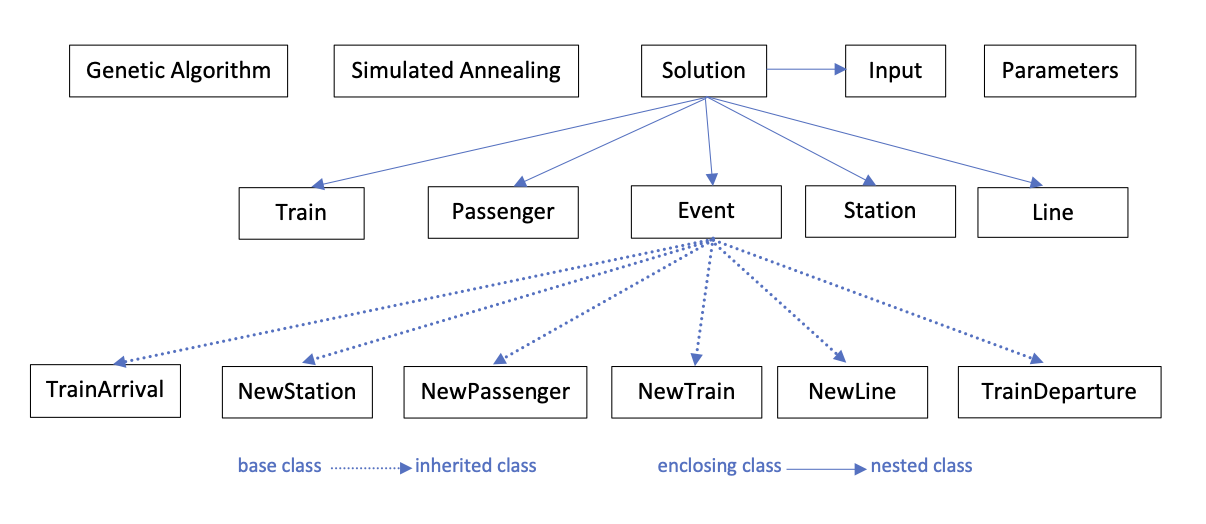
\includegraphics[scale = 0.8]{pictures/class_hierarchy.png}
    \caption{Class hierarchy}
\end{figure}

The class hierarchy of the main program can be seen in the figure above. Both optimization methods have their own class. Additionally, there is a class for parameters and a large class for the general solution. The solution class has many nested classes, which only need to be accessed while computing a solution. The class Event is the base class to many other classes, each describing an event. They all inherit from the same base class because there are things that all events have in common. The trains, passengers, stations, and lines are shared by all solutions. They are reset between the calculation of two different solutions. The same holds for the events that create a new station, passenger, train, or line. The events TrainArrival and TrainDeparture are always deleted after one solution.


\subsection{$Solution$}
$Solution$ is the class for a general solution. When initialized, it takes a set of parameters and automatically computes the number of time steps and whether it succeeds in getting all passengers to their target station.

Pseudocode for calculation of general solution:
\lstset {language=C++}
\begin{lstlisting}
    events = input_events
    overfilled = false
    while(!overfilled)
    {   
        e = events.next()
        events.remove(e)
        overfilled = e.run(events)
    }
\end{lstlisting}

On the first line a list of events is declared and set to contain the events from the input. Then the Boolean overfilled is set to false and events are executed until the system is overfilled. The most important part here happens in the $run()$ method, which is different for each event. It returns true if the system is overfilled after the current event and false otherwise. It also adds new events to the events list if new events are created. This happens for example after the event $TrainDeparture$, where a new $TrainArrival$ is added. This will be described separately for each type of event:

\subsubsection{NewObject}
The appearance of an object (train, station, passenger, line) is an event. Here, $run()$ mainly initializes the object and adds it to necessary lists. For lines and trains, the line or train is added to the system immediately after this.

\subsubsection{NewTrain}
New train adds a new train to the simulation. If there are lines which do not have any trains yet, the train is added to one of those. If there are no such lines, the train is added to the line which currently has the most stations per train.

\subsubsection{NewLine}
When a new line is created, all new stations are added to it. In addition to this, an equal number of stations which already are on a line is added.

\subsubsection{TrainArrival}
When a train arrives at a station, multiple things happen. Firstly, the train is registered at the station. Next, it is decided which passengers should leave the train and which passengers should board. It never makes sense for a passenger to stay on a train if it has the option to leave the train to a station of the correct type (i.e. the type of station where the passenger was headed). Therefore, this will be done automatically, no matter what the parameters for that action say. The same thing happens with passengers who should board or leave a train if that action leads to an overfilled train or station. In every other case, this is where the parameters that can be adapted by the two optimization methods come into play. There are eight parameters in total, four deciding when a passenger should board a train and the other four when it should leave the train.

\subsubsection{TrainDeparture}
The most important thing that happens when a train departs is that a new train arrival and departure are scheduled, i.e. added to the list of events.


\subsection{Station, Passenger, Train, Line}
The clear objects in the problem of course also get their own classes. All these classes have properties such as their id and time of appearance.

\subsection{Optimization methods}
The optimization methods have been implemented as described in the theory chapter, where their pseudocode can be found.

\section{New Line and Line Changes}
Creating a new line comes with many challenges. Firstly, one has to decide on the stations which the new line should cover. After that the order in which the stations on the line are visited has to be determined. In many cases, it makes sense to just connect the stations in an order which minimizes the total time it takes for a train to make a round on the line. This is an optimization problem of its own.

\newpage
\chapter{Results}
The two algorithms were evaluated based on their performance in optimizing train networks. 80 different random input files were created.

The following table and pie chart show how many of the 80 tests ended in a win by which method:

\begin{table}[h]
    
    \begin{center}
        \begin{tabular}{|c|c|c|c|c|}
            \hline
            \rowcolor{lightgray}
            SA & SA (time) & Draw & GA (time) & GA \\
            \noalign{\hrule height 1.5pt}
            \cellcolor[HTML]{6A99D0}\color{white}30 & \cellcolor[HTML]{A5C2E3}\color{white}5 & \cellcolor[HTML]{A5A5A5}\color{white}38 & \cellcolor[HTML]{E9B38A}\color{white}1 & \cellcolor[HTML]{DE8244}\color{white}6 \\
            \hline
        \end{tabular}
    \end{center}
    \caption{Results table}
    \end{table}


\begin{center}
\begin{figure}[h]
    \centering
    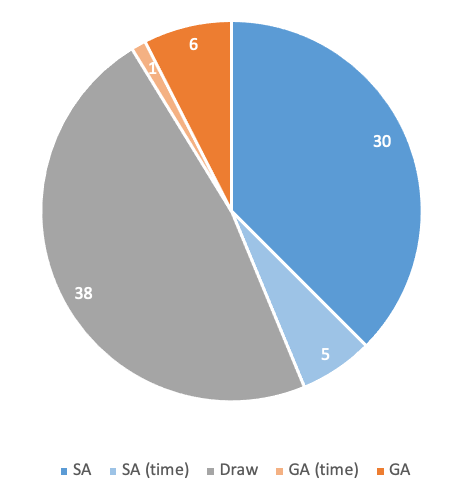
\includegraphics[scale = 1]{pictures/results.png}
    \caption{Results pie chart}
    \label{}
\end{figure}

\end{center}

SA stands for simulated annealing and GA for genetic algorithm. (time) indicates that both methods have transported the same number of passengers, but the winning method took less time. The average number of passengers transported by the solutions found by simulated annealing and the genetic algorithm were $1519$ and $1480$ respectively. Both values were rounded to the closest integer.

\chapter{Discussion}

\section{Description of the Results}
The results show that the two methods have performed similarly well. This is indicated by the fact that the solutions found by the two methods performed exactly the same way in almost half of the tests. Additionally, the difference between the average number of transported passengers is relatively small. Still, simulated annealing has performed slightly better. It is important to note that in most cases, the differences were not very large. The exact results for all tests can be found in the appendix.


\section{Possible Explanations}
The similar results might be due to the fact that the methods could only choose when passengers would board or leave trains. Other parts of the solution were not adapted by the two optimization methods. This has led to the fact that there were many sets of parameters leading to the same solution. A possible explanation for the better performance of simulated annealing could be that the method only actively works with one solution, but that solution is often one of the best solutions it has encountered. A genetic algorithm works with many different solutions, which also includes many worse ones, especially in the beginning. Once a genetic algorithm encounters a solution which is much better than all the solutions it has seen so far, it takes multiple generations for its parameters to be integrated into most individuals of its population. When simulated annealing finds a better solution, it starts working from there instead of still considering multiple worse previous solutions. This effect is increased by the fact that the methods only had 200 solutions to try out and the genetic algorithm may have wasted a few of those on some generations of bad solutions despite already knowing some better ones.

\section{Future Work}
As a next step, one could parametrize more of the solution to let the optimization methods decide about more parts. This will lead to many more possible solutions. It will also be much less likely for two methods to reach exactly the same answer. It would be interesing to see if simulated annealing would still perform better under those conditions.

\chapter{Conclusion}
The program to compare the two algorithms was implemented and tested. The program runs without issues and the two methods are adapting the solutions and reaching relatively good results. The two methods have been compared in their performance. The main objectives of this project have been met.

The two methods have led to similar results with few significant differences. Overall, the method simulated annealing has performed a bit better. In conclusion, it can be said that both methods can achieve similarly good answers to optimization problems. Additional testing with more parameters might be required to determine which method is really better for this problem. 

\newpage


\chapter*{Acknowledgements}

I would like to thank my family for their support while working on this project. I would also like to thank the Swiss Olympiad in Informatics for giving students great opportunities to explore computer science outside of school and coming up with the train network problem. I would especially like to thank Benjamin Schmid for creating the visualization for this problem. Finally, I would like to thank my supervisor Stefan Rothe for his invaluable support throughout this project.

\chapter*{Declaration of Authorship}

I, Ema Skottova, hereby confirm that this paper is wholly my own work unless otherwise acknowledged. Other sources have been documented.

\listoffigures

\listoftables

All tables and figuers were created by the author. The picture on the cover page and figure 2.1 were created using the visualization of the train network problem created by Benjamin Schmid.

\printbibliography

\chapter*{Electoric Version}
An electronic version of this paper as well as the programs can be found at \url{https://github.com/eskottova/MaturaProject}.


\chapter*{Data}
\begin{center}
    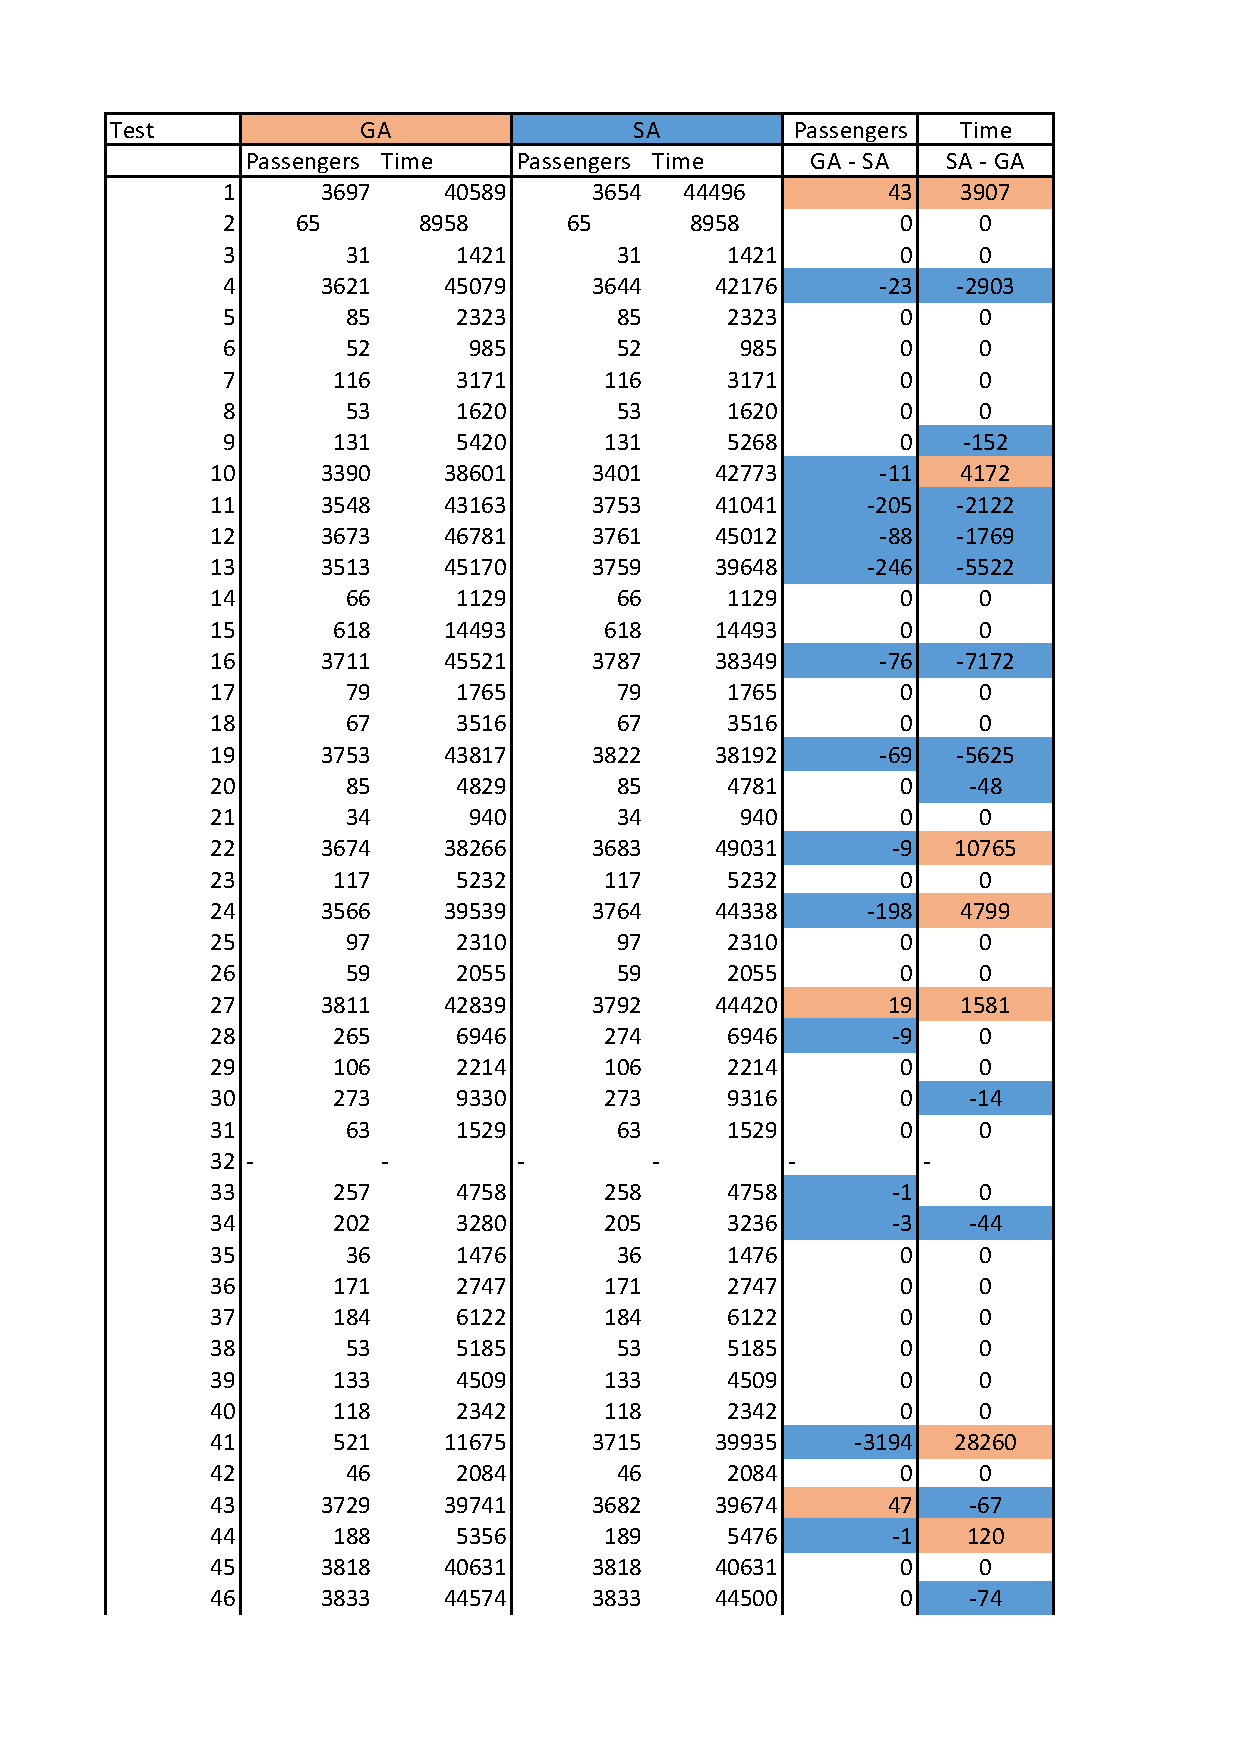
\includegraphics[scale = 0.8]{pictures/results1.pdf}
    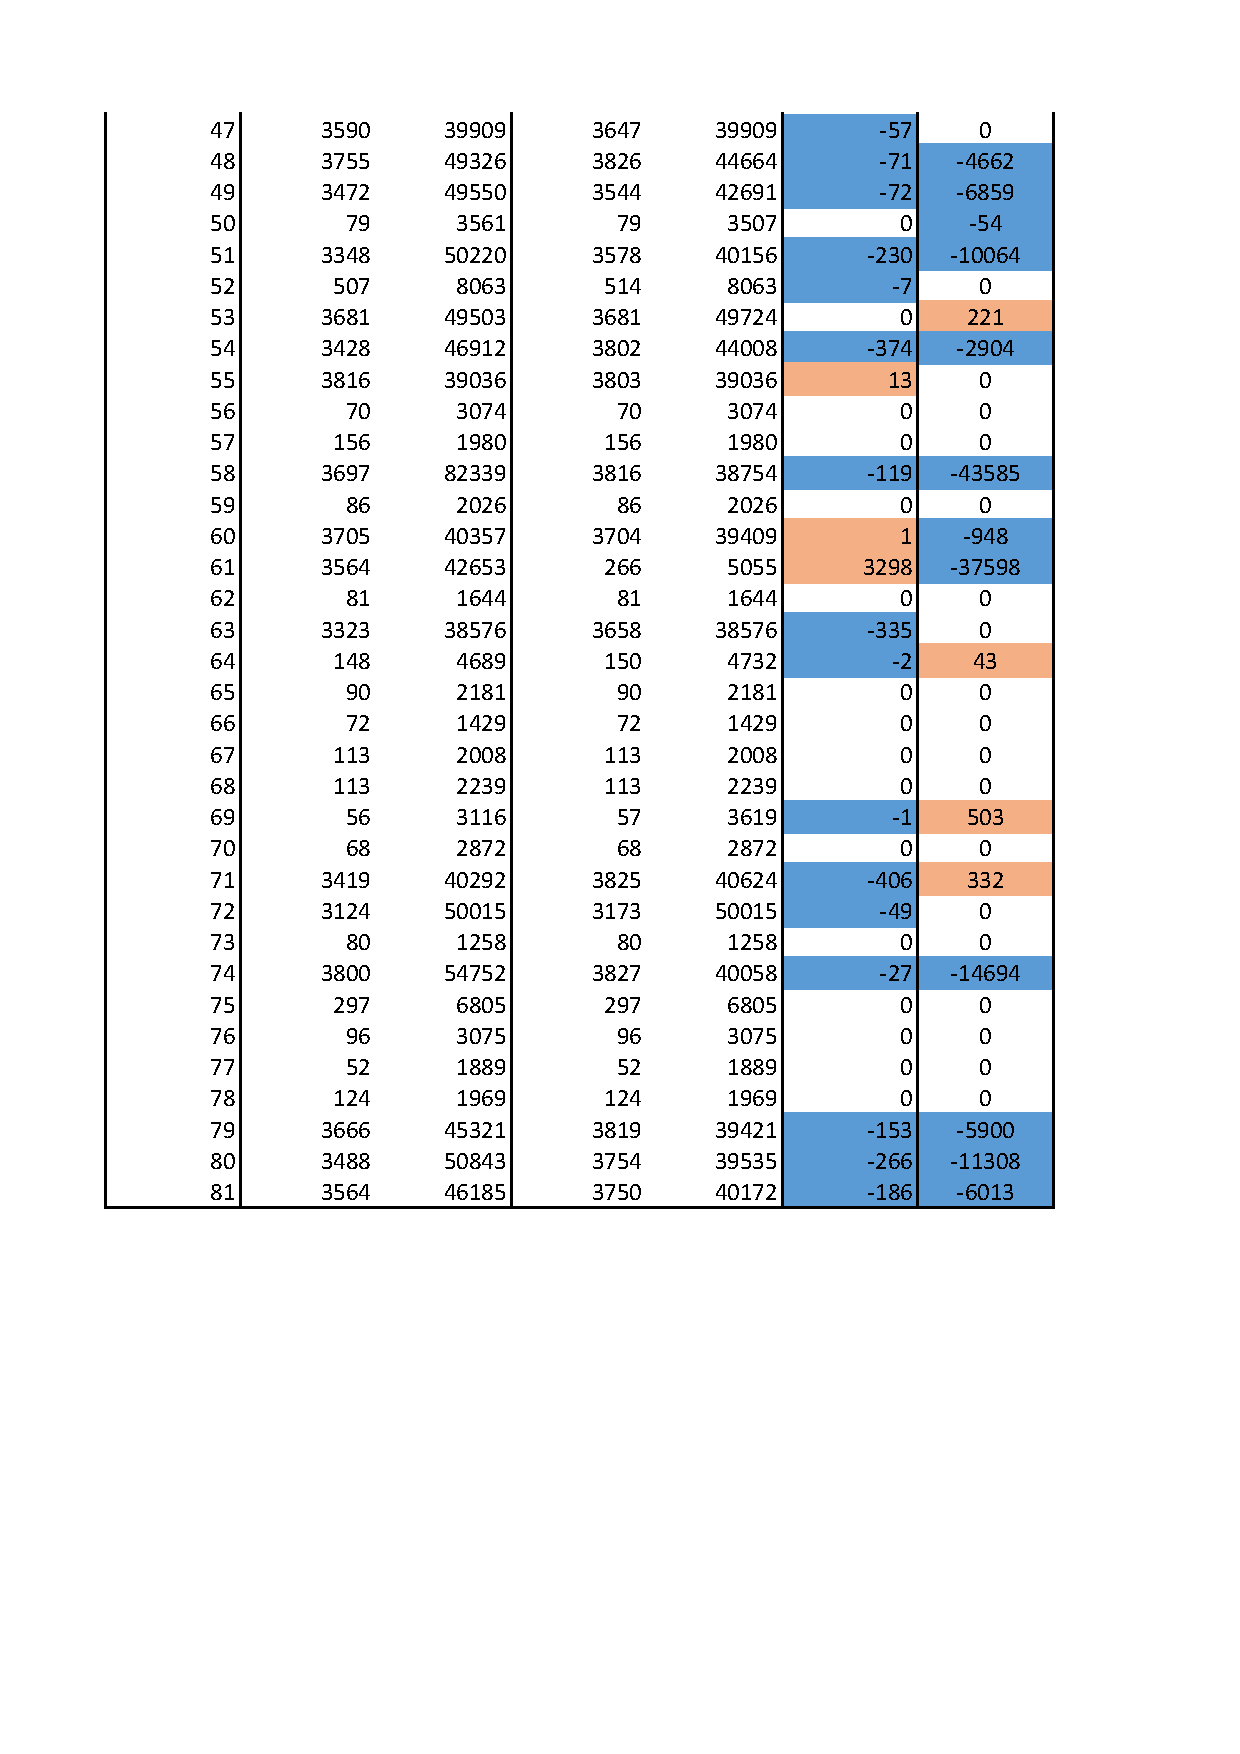
\includegraphics[scale = 0.8]{pictures/results2.pdf}
\end{center}
\end{document}


